% ju 28-Nov-24 SP-HU-AU-notiz.tex
\documentclass{vorlage-design-main}
% Verwenden von fontspec und unicode-math für XeLaTeX oder LuaLaTeX

%% Ganze Überschrift
\title{Sicherheitsprüfung, Hauptuntersuchung und Abgasuntersuchung}
%% Kürzerer Titel
\runningtitle{SP - HU - AU}
\author{Jan Unger}
\date{\today}

%% Referenzen
\addbibresource{literatur.bib}

\begin{document}

\maketitle

\begin{abstract}
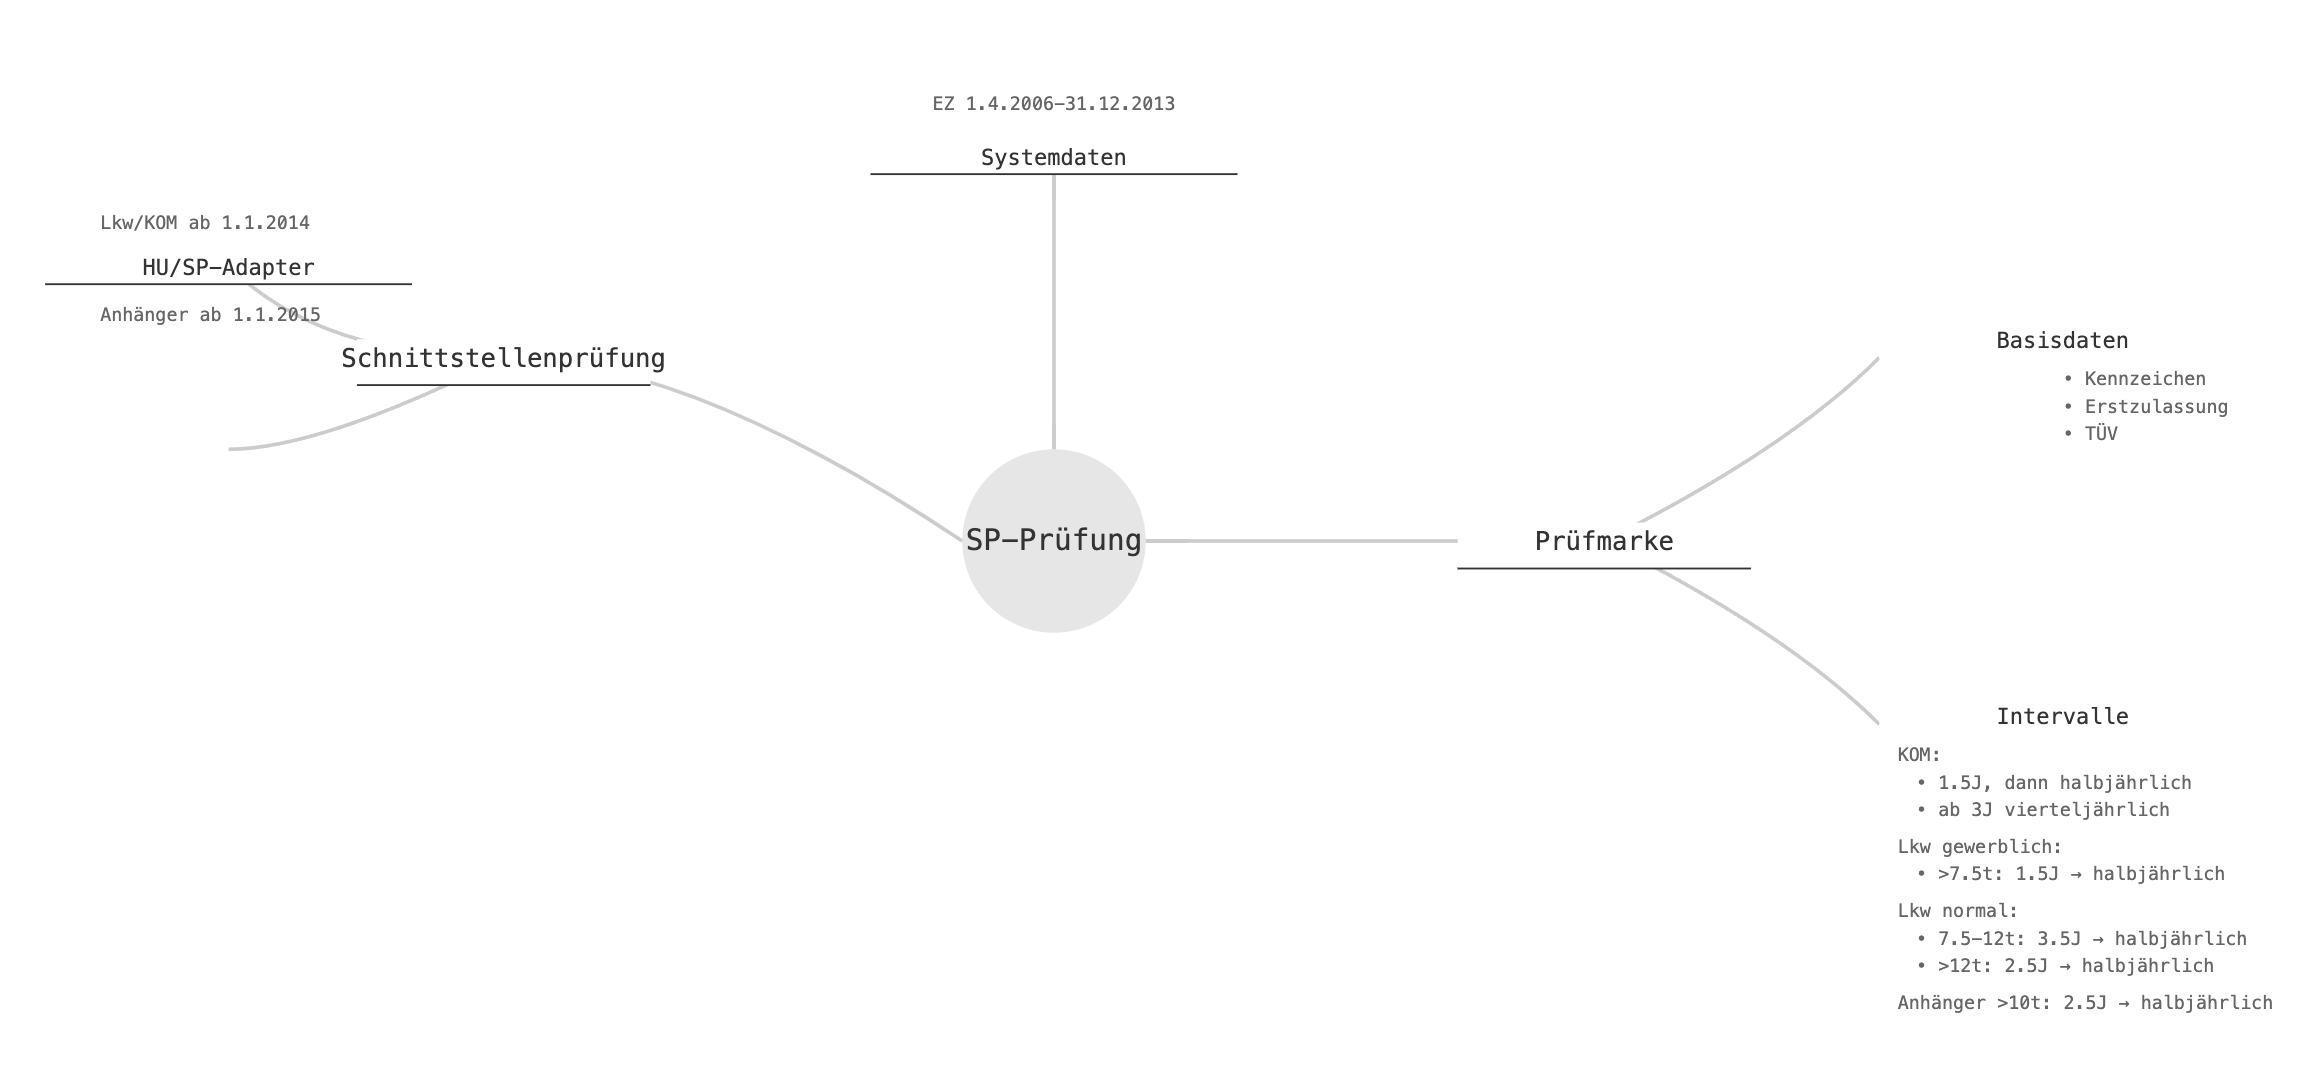
\includegraphics[width=0.9\textwidth]{images/SP-Durchfuehrung-Mindmap.png}


\end{abstract}

\newpage

\subsection{SP}\label{sp}

Letzte Bearbeitung am: 26.11.2024

\textbf{Checkliste für SP-Durchführung}:

\begin{itemize}

\item[$\square$]
  Vorbereitung: Prüfbuch, PC, TV, AÜK Plus und MAHA

  \begin{itemize}

  \item[$\square$]
    Kennzeichen und Kilometer
  \item[$\square$]
    Fahrzeugschein (Audits)
  \item[$\square$]
    Probefahrt (mind. 8 km/h)
  \end{itemize}
\item[$\square$]
  Schnittstellenprüfung: HU/SP-Adapter

  \begin{itemize}

  \item
    Erstzulassung ab 1.1.2014 (Lkw und KOM) und 1.1.2015 (Anhänger)
  \end{itemize}
\item[$\square$]
  Systemdatenprüfung:

  \begin{itemize}

  \item
    Erstzulassung 1.4.2006 bis 31.12.2013
  \end{itemize}
\item[$\square$]
  MAHA: Prüfung neu anlegen, Stammdaten/Komplettdatensatz laden und
  Daten erfassen

  \begin{itemize}

  \item[$\square$]
    Weiter / Messung starten
  \end{itemize}
\item[$\square$]
  Bremswirkungsprüfung
\item[$\square$]
  MAHA: Messung beenden und speichern
\item[$\square$]
  AÜK Plus: Daten erfassen
\item[$\square$]
  Sicht-, Funktions- und Wirkungsprüfung
\item[$\square$]
  AÜK Plus: Dokumentation
\item[$\square$]
  Prüfnachweis (Unterschrift, Siegel, Prägung)
\item[$\square$]
  SP-Prüfmarke

  \begin{itemize}

  \item[$\square$]
    Kennzeichen
  \item[$\square$]
    Erstzulassung (Neuwagen)
  \item[$\square$]
    TÜV
  \item[$\square$]
    nächste SP

    \begin{itemize}

    \item[$\square$]
      KOM

      \begin{itemize}

      \item
        erste SP: nach 1,5 Jahren
      \item
        Folge-SPs: bis 3. Jahr halbjährlich und ab 3. Jahr
        vierteljährlich
      \end{itemize}
    \item[$\square$]
      Lkw \textgreater{} 7,5 t (gewerblich vermietet): nach 1,5 Jahren,
      halbjährlich
    \item[$\square$]
      Lkw 7,5 t - 12 t: nach 3,5 Jahren, halbjährlich
    \item[$\square$]
      Lkw \textgreater{} 12 t: nach 2,5 Jahren, halbjährlich
    \item[$\square$]
      Anhänger \textgreater{} 10 t: nach 2,5 Jahren, halbjährlich
    \end{itemize}
  \end{itemize}
\end{itemize}

Netzwerkkontrolle: USB-Stick/Daten-Backup oder USB-Kabel und WLAN
(wlan\_sws\_spezial03)

\newpage

SP-Durchführung:

\begin{enumerate}
\def\labelenumi{\arabic{enumi}.}
\item
  \textbf{Vorbereiten der SP}:

  \begin{itemize}

  \item
    PC und TV
  \item
    Software: AÜK Plus und MAHA
  \item
    Kennzeichen und Kilometer, Prüfbuch, Fahrzeugschein (Audits)
  \item
    Schnittstellenprüfung: HU-Adapter (Erstzulassung ab 1.1.2014 (Lkw
    und KOM) und 1.1.2015 (Anhänger))
  \item
    Systemdatenprüfung (Erstzulassung 1.4.2006 bis 31.12.2013)
  \item
    Probefahrt (mind. 8 km/h)
  \end{itemize}
\item
  \textbf{MAHA: (4) Prüfung neu anlegen}

  \begin{itemize}

  \item
    Stammdaten / Komplettdatensatz laden und Fahrzeug aus Liste
    auswählen
  \item
    Datenübersicht: (Kontrolle \& Eingabe)

    \begin{itemize}

    \item
      Kennzeichen
    \item
      Achsen: Anzahl
    \item
      VIN
    \item
      Fahrzeugart und Klasse
    \item
      Kilometer
    \item
      Prüfer
    \end{itemize}
  \item
    Weiter / \textbf{Messung starten}
  \end{itemize}
\item
  \textbf{Bremswirkungsprüfung}: Prüffahrzeug achsweise über den
  Rollenbremsprüfstand fahren.

  \begin{itemize}

  \item
    Bus in Rolle fahren und Automatik ausschalten (Fernbedienung: rote
    Stop-Tasten)
  \item
    Bremsen: Fernbedienung Zahl (1/2/3) und BBA/FBA und * (speichern)
  \item
    Anwenden der Bezugsbremskräfte (Bremsreferenzwerte)

    \begin{itemize}

    \item
      Mindestbremskraft: bei einem Mindestbremsdruck von 1,7 bar
    \end{itemize}
  \item
    Hochrechnung (konventionell)
  \end{itemize}
\item
  \textbf{MAHA: (4) Messung beenden und speichern}
\item
  \textbf{Erfassen der relevanten Daten:} (AÜK Plus)

  \begin{itemize}

  \item
    Sicherheitsprüfung (neu)
  \item
    Kennzeichen und \textbf{Tab-Taste} drücken
  \item
    FSD Vorgaben-Prüfung starten (Systemverbauprüfung und
    Bezugsbremskräfte)
  \item
    Import: Bremswerte
  \item
    Fahrzeug- und Prüfungsdaten kontrollieren
  \item
    \textbf{km-Stand} und \textbf{Prüfdatum + Zeit} und \textbf{letzte
    HU}
  \item
    Fachkraft und verantwortliche Person eintragen
  \item
    \textbf{Prüfungsart:} Sicherheitsprüfung / Nachprüfung
  \item
    Bremse: Bremswerte berechnen
  \item
    Prüfmittel
  \end{itemize}
\item
  \textbf{Sicht- / Funktions- / Wirkungsprüfung}

  \begin{itemize}

  \item
    Fahrgestell / Fahrwerk / Aufbau / Verbindungseinrichtung
  \item
    Lenkung
  \item
    Reifen / Räder
  \item
    Bremsanlage
  \end{itemize}
\item
  \textbf{Dokumentation der Sicherheitsprüfung:} (AÜK Plus)

  \begin{itemize}

  \item
    Mängel festgestellt?
  \item
    \textbf{Mängel}: ohne Mängel / mit Mängeln / verkehrsunsicher
  \item
    \textbf{Die o. g. Mängel wurden}

    \begin{itemize}

    \item
      sofort behoben
    \item
      nicht behoben
    \end{itemize}
  \item
    \textbf{Ergebnis}:

    \begin{itemize}

    \item
      Prüfmarke zugeteilt
    \item
      Prüfmarke nicht zugeteilt, Nachprüfung erforderlich
    \item
      Prüfmarke entfernt
    \end{itemize}
  \item
    \textbf{Ablauf der Frist für die nächste SP}
  \item
    Check und Prüfung abschließen und Prüfnachweis drucken
  \end{itemize}
\item
  \textbf{Prüfnachweis unterschreiben, siegeln und prägen}

  \begin{itemize}

  \item
    \textbf{Siegel}: SP-Prüfmarke (Siegeljahr), anerkannte SP-Werkstatt
  \item
    \textbf{Prüfbuch}: Stempel (Firmenadresse und Kontroll-Nr. der
    anerkannten Werkstatt) und Unterschrift
  \item
    \textbf{Prüfprotokoll Sicherheitsprüfung}: Stempel (Firmenadresse)
    und Unterschrift und Nachweis-Siegel mit Prägenummer (Prägezange)
    und KOM (WG-Nr.)
  \end{itemize}
\item
  \textbf{Anbringen der SP-Prüfmarke am Prüffahrzeug}
\item
  \textbf{Drucksicherungsprüfung}

  \begin{itemize}

  \item
    Förderleistung / Füllzeit
  \item
    Dichtheit der Anlage (bis Abschaltdruck befüllen, Bremszylinderdruck
    (3 bar), Beruhigungszeit (1 Min.), in 3 Min. nicht mehr als 0,4 bar)
  \item
    Drucksicherungsfunktion (Regel ≥ 4,5 bar)
  \item
    Abreißsicherungsfunktion (nur bei Anhängervorrichtung)

    \begin{itemize}

    \item
      Bei \textbf{Abriss der Vorratsleitung} (Rot) darf kein ungewolltes
      >>Einbremsen<< der Federspeicher-Bremszylinder (Motorwagen)
      erfolgen (Rückschlagventil im Kreis 3)
    \item
      Am Anhänger muss die BBA/FBA aufgrund der entlüfteten
      Vorratsleitung selbstständig in Vollbremsung gehen
    \item
      Bei \textbf{Abriss der Bremsleitung} (Gelb) muss bei voller
      Bremsbetätigung der BBA (Motorwagen) der Druck in der
      Vorratsleitung zum Anhänger in 2 Sekunden auf 1,5 bar sinken und
      somit die selbstständige Bremsung des Anhängers auslösen
    \end{itemize}
  \item
    Löseventil am Anhänger (Rangiervorgänge)

    \begin{itemize}

    \item
      Das an einem angekuppelten Anhänger betätigte Löseventil muss bei
      Druckaufbau über die Vorratsleitung selbstständig wieder in
      Betriebsstellung gehen
    \end{itemize}
  \item
    Abstuftbarkeit (max. 0,3 bar) und Zeitverhalten bis Vollbremsung
    (unmittelbar)
  \end{itemize}
\end{enumerate}

\textbf{Hinweis}: Alte SPs / HUs (Was wurde gemacht?) und zeitlicher
Abstand zwischen zwei SPs beachten (mind. 30 Min.)

\subsubsection{Inspektionsablauf zur SP}\label{inspektionsablauf-zur-sp}

\subsubsection{SP - Ablaufdiagramm}\label{sp---ablaufdiagramm}

\begin{figure}
\centering
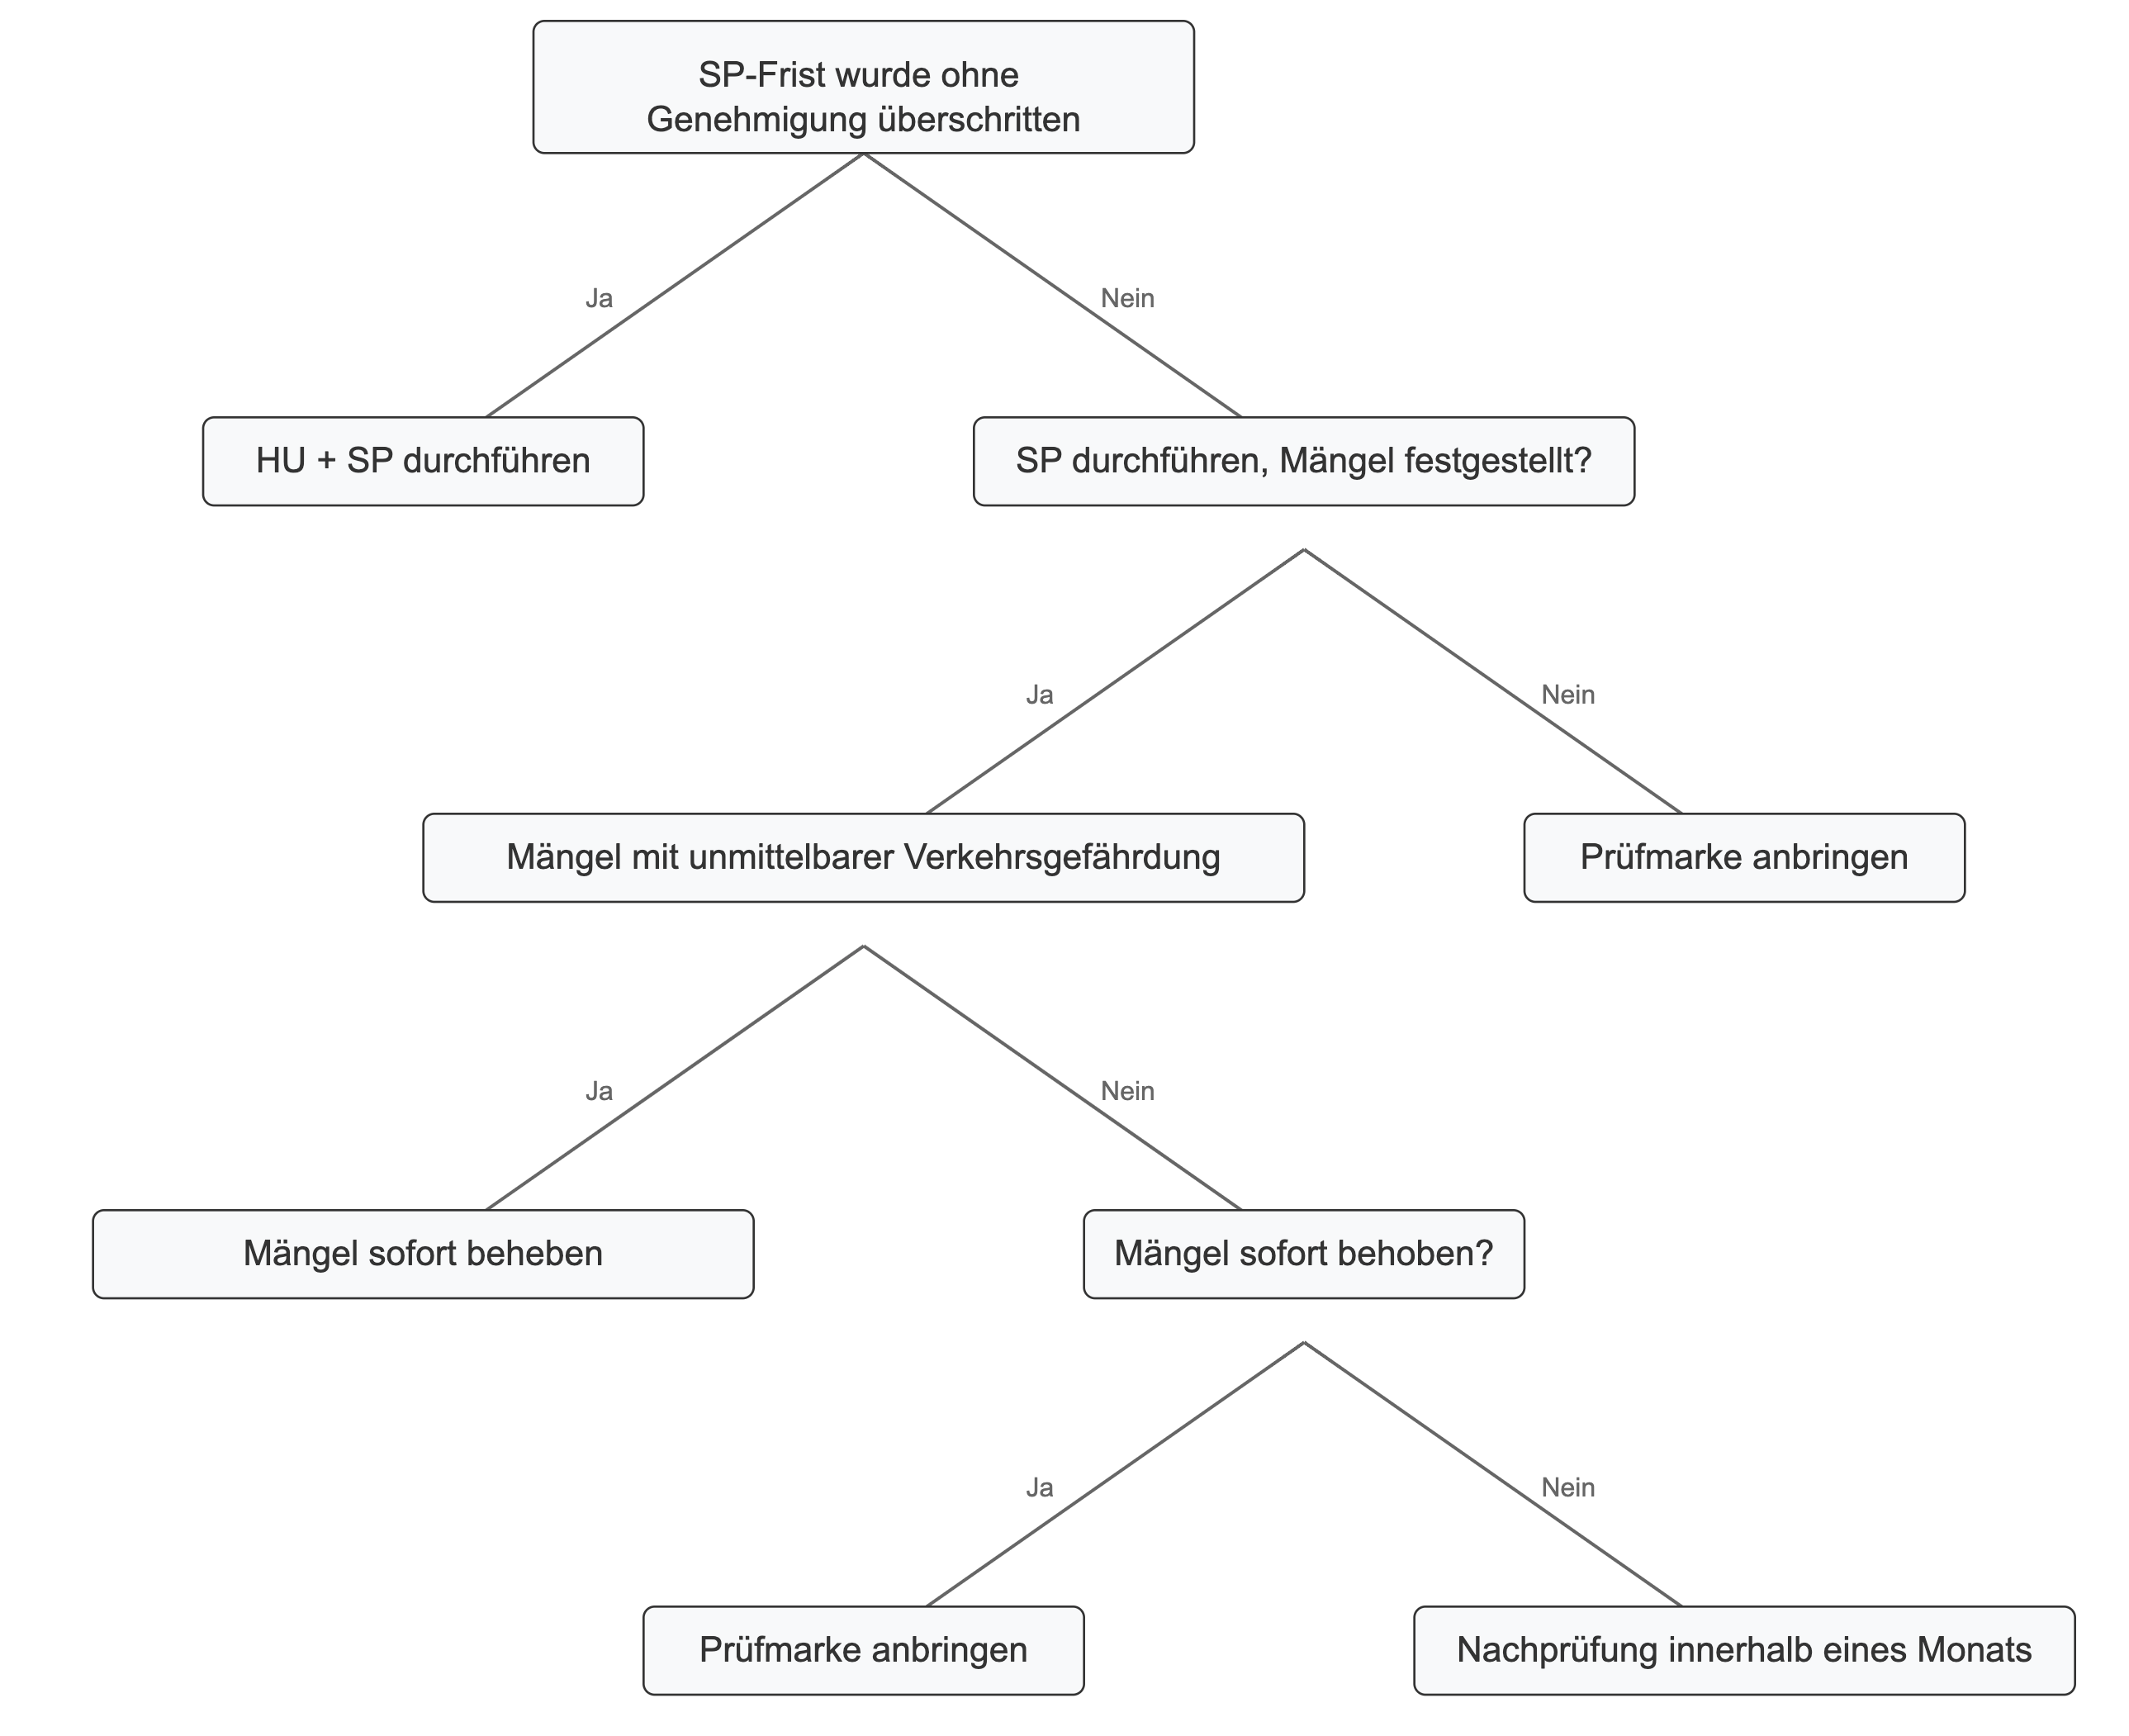
\includegraphics[width=0.8\linewidth,keepaspectratio]{images/SP-Ablaufdiagramm.png}
%\floatnotes{}
%\label{fig:}
\caption{SP Ablaufdiagramm}
\end{figure}

\begin{table}[ht]
  %\caption{}
  %\label{tab:my-table}
  \begin{tabular}{@{}lll@{}}
\toprule
Code
 &
Mängelkategorie
 &
Ergebnis
 \\
\midrule[\heavyrulewidth]
1 & Ohne erkennbare Mängel & Prüfmarke zugeteilt \\
2 & Mängel festgestellt & Prüfmarke nicht zugeteilt, Nachprüfung
erforderlich \\
3 & Unmittelbare Verkehrsgefährdung & Prüfmarke entfernt \\
\bottomrule
\end{tabular}%
\end{table}

\begin{enumerate}
\def\labelenumi{\arabic{enumi}.}

\item
  \textbf{Prüfungsart}

  \begin{itemize}

  \item
    1 Sicherheitsprüfung
  \item
    2 Nachprüfung zu SP d.~aaSoP / PI
  \item
    3 Nachprüfung zu SP d.~anerk. Werkst.
  \end{itemize}
\item
  \textbf{Die o. g. Mängel wurden}

  \begin{itemize}

  \item
    1 sofort behoben
  \item
    2 nicht behoben
  \end{itemize}
\end{enumerate}

\subsubsection{Fristen für Sicherheitsprüfungen nach
Fahrzeugtyp}\label{fristen-fuer-sicherheitspruefungen-nach-fahrzeugtyp}

Abbildung 1-15: SP-Fristen untersuchungspflichtiger Nutzfahrzeuge zeigt
eine Übersicht der Prüfintervalle für Kraftomnibusse (KOM),
Kraftfahrzeuge zur Güterbeförderung (Lkw) und Anhänger. {[}1, S. 38{]}

\begin{table}[ht]
  %\caption{}
  %\label{tab:my-table}
  \begin{tabular}{@{}lll@{}}
\toprule
Fahrzeugtyp
 &
Erste SP
 &
Folgende SPs
 \\
\midrule[\heavyrulewidth]
KOM & nach 1,5 Jahre & 1.-3. Jahr: Halbjährlich, ab 3. Jahr:
Vierteljährlich \\
LKW \textgreater{} 7,5 t (gewerblich vermietet) & nach 1,5 Jahre &
Halbjährlich \\
LKW 7,5 t - 12 t & nach 3,5 Jahre & Halbjährlich \\
LKW \textgreater{} 12 t & nach 2,5 Jahre & Halbjährlich \\
Anhänger \textgreater{} 10 t & nach 2,5 Jahre & Halbjährlich \\
\bottomrule
\end{tabular}%
\end{table}

\subsubsection{Ausnahmeregelungen zu den
SP-Fristen}\label{ausnahmeregelungen-zu-den-sp-fristen}

\begin{table}[ht]
  %\caption{}
  %\label{tab:my-table}
  \begin{tabular}{@{}ll@{}}
\toprule
Situation
 &
Regelung
 \\
\midrule[\heavyrulewidth]
Vorzeitige SP-Durchführung & Bis zu 1 Monat vor Fälligkeit möglich,
nächste SP-Frist unverändert \\
Vorziehen der HU & Möglich, SP-Frist wird angepasst \\
HU-Fristüberschreitung & Bis 2 Monate: normale HU, Ab 3. Monat:
vertiefte HU (HU+) \\
Saisonkennzeichen/Außerbetriebsetzung & HU/SP-Termine werden
übersprungen \\
\bottomrule
\end{tabular}%
\end{table}

\begin{enumerate}
\def\labelenumi{\arabic{enumi}.}

\item
  \textbf{Vorzeitige SP-Durchführung:}

  \begin{itemize}

  \item
    SP-pflichtige Nutzfahrzeuge können einen Monat vor dem auf der
    SP-Prüfmarke ausgewiesenen Monat zur SP vorgeführt werden.
  \item
    Der vorgeschriebene Zeitabstand für die nächste SP ändert sich
    dadurch nicht.
  \end{itemize}
\item
  \textbf{Vorziehen der HU:}

  \begin{itemize}

  \item
    Es besteht die Möglichkeit, die HU vorzuziehen, z.B. wenn
    Sattelzugmaschine und zugehöriger Anhänger unterschiedliche
    HU-Termine haben.
  \item
    Der HU-Prüfer muss mit dem Abschluss der HU auch die Frist zur
    nächsten SP anpassen.
  \item
    Er verklebt hierzu eine neue SP-Prüfmarke ohne Durchführung einer
    erneuten SP.
  \end{itemize}
\item
  \textbf{Fristüberschreitung einer fälligen HU:}

  \begin{enumerate}
  \def\labelenumii{\arabic{enumii}.}

  \item
    \textbf{Fristbeginn}:

    \begin{itemize}

    \item
      Die Frist für die nächste HU beginnt mit dem Monat und Jahr der
      letzten HU.
    \end{itemize}
  \item
    \textbf{Fristüberschreitung}:

    \begin{itemize}

    \item
      Bis zu 2 Monate nach Fristablauf: >>normale<< HU
    \item
      Ab dem 3. Monat: >>vertiefende<< HU (HU+), die Pflicht- und
      Ergänzungsuntersuchungen umfasst
    \end{itemize}
  \item
    \textbf{Neue Frist:}

    \begin{itemize}

    \item
      Beginnt immer mit dem Monat der HU-Durchführung
    \item
      Volle Frist bis zur nächsten fälligen HU wird gewährt
    \end{itemize}
  \item
    \textbf{Prüfplaketten:}

    \begin{itemize}

    \item
      Neue HU-Prüfplakette wird zugeteilt
    \item
      Neue SP-Prüfmarke (Sicherheitsprüfung) muss vom HU-Prüfer ohne
      SP-Durchführung angebracht werden
    \item
      Dies wird im HU-Bericht vermerkt
    \end{itemize}
  \end{enumerate}
\end{enumerate}

\subsubsection{Fristenregelung mit Saisonkennzeichen bzw.
Außerbetriebsetzung}\label{fristenregelung-mit-saisonkennzeichen-bzw.-ausserbetriebsetzung}

\begin{enumerate}
\def\labelenumi{\arabic{enumi}.}

\item
  \textbf{Während der Saisonkennzeichen-Zeit oder Außerbetriebsetzung:}

  \begin{itemize}

  \item
    HU- und SP-Termine werden übersprungen.
  \item
    Diese Zeit wird als >>Saisonkennzeichen bzw. Außerbetriebsetzung<<
    gekennzeichnet.
  \end{itemize}
\item
  \textbf{Bei Wiederinbetriebnahme:}

  \begin{itemize}

  \item
    Dies wird als >>HU-/SP-Durchführung mit neuen Fristen<< markiert.
  \item
    \textbf{Folgen}

    \begin{itemize}

    \item
      Die HU-Durchführung wird mit einer SP verbunden.
    \item
      Die HU-Prüfplakette wird auf den Durchführungstermin geklebt.
    \item
      Eine neue SP-Prüfmarke wird zugeteilt.
    \end{itemize}
  \end{itemize}
\end{enumerate}

\subsubsection{Fristüberschreitungen für LKW / KOM bei der
SP}\label{fristueberschreitungen-fuer-lkw-kom-bei-der-sp}

\begin{enumerate}
\def\labelenumi{\arabic{enumi}.}

\item
  \textbf{Fristüberschreitung mit Bestätigung im SP-Prüfprotokoll:}

  \begin{itemize}

  \item
    LKW: SP nach 7 Monaten statt 6 zur letzten HU
  \item
    KOM: SP nach 4 Monaten statt 3 zur letzten HU
  \item
    \textbf{Folgen}:

    \begin{itemize}

    \item
      Rechtzeitige SP-Beauftragung
    \item
      SP-Durchführung mit Vermerk im SP-Protokoll
    \end{itemize}
  \end{itemize}
\item
  \textbf{Fristüberschreitung ohne Bestätigung im SP-Protokoll:}

  \begin{itemize}

  \item
    LKW: SP nach 7 Monaten statt 6 zur letzten HU
  \item
    KOM: SP nach 4 Monaten statt 3 zur letzten HU
  \item
    HU/SP-Durchführung mit neuen Fristen
  \item
    \textbf{Folgen}:

    \begin{itemize}

    \item
      Keine rechtzeitige SP-Beauftragung
    \item
      HU-Durchführung verbunden mit einer SP
    \item
      HU-Prüfplakette wird auf den Durchführungstermin geklebt
    \item
      Neue SP-Prüfmarke wird zugeteilt
    \end{itemize}
  \end{itemize}
\end{enumerate}

\subsubsection{Nicht durchgeführte SP bei
HU-Vorführung}\label{nicht-durchgefuehrte-sp-bei-hu-vorfuehrung}

\begin{enumerate}
\def\labelenumi{\arabic{enumi}.}

\item
  \textbf{Nicht durchgeführte SP bei HU-Vorführung:}

  \begin{itemize}

  \item
    Die SP zwischen zwei HU kann nicht nachgewiesen werden
  \item
    Bei der nächsten HU wird eine kombinierte HU/SP durchgeführt
  \item
    \textbf{Folgen:}

    \begin{itemize}

    \item
      HU-Durchführung wird mit einer SP verbunden
    \item
      Die SP wird mit einem SP-Prüfprotokoll dokumentiert
    \item
      Eine neue SP-Prüfmarke wird zugeteilt
    \end{itemize}
  \end{itemize}
\end{enumerate}

\subsubsection{Fristüberschreitung für die Nachprüfung der
SP-Mängelbeseitigung}\label{fristueberschreitung-fuer-die-nachpruefung-der-sp-maengelbeseitigung}

\begin{enumerate}
\def\labelenumi{\arabic{enumi}.}

\item
  \textbf{Regelfall für die Nachprüfung mit SP-Prüfprotokoll:}

  \begin{itemize}

  \item
    Vorlage des SP-Prüfprotokolls zur Nachprüfung
  \item
    Nachprüfung der SP innerhalb eines Monats (i.d.R. 30 Tage)
  \item
    SP-Prüfmarke wird auf den ursprünglichen Termin geklebt
  \item
    Keine zusätzlichen Mängel festgestellt
  \end{itemize}
\item
  \textbf{Fristüberschreitung \textgreater{} 1 Monat mit
  SP-Prüfprotokoll:}

  \begin{itemize}

  \item
    Vorlage des SP-Prüfprotokolls zur Nachprüfung
  \item
    Durchführung einer neuen SP
  \item
    SP-Prüfmarke wird auf den ursprünglichen Termin geklebt
  \end{itemize}
\item
  \textbf{Fristüberschreitung \textgreater{} 1 Monat oder fehlendes
  SP-Prüfprotokoll:}

  \begin{itemize}

  \item
    Keine Vorlage des SP-Prüfprotokolls
  \item
    HU-Durchführung verbunden mit einer SP
  \item
    HU-Prüfplakette wird auf den Durchführungstermin geklebt
  \item
    Neue SP-Prüfmarke wird zugeteilt
  \item
    Neue Fristen für HU und SP beginnen
  \end{itemize}
\end{enumerate}

\subsubsection{Beispiele nächste SP}\label{beispiele-naechste-sp}

\textbf{Beispiel 1 nächste SP}: KOM

\begin{itemize}

\item
  Erstzulassung: 01/2011
\item
  letzte HU: 12/2023
\item
  letzte SP: 03/2024
\item
  Prüfdatum SP: 28.6.24 (aktuelle SP: 06/2024)
\item
  Ablauf der Frist für die nächste SP: 09/2024
\end{itemize}

\textbf{Beispiel 2 nächste SP}: KOM

\begin{itemize}

\item
  Erstzulassung: 10/2011
\item
  letzte HU: 10/2023
\item
  letzte SP: 04/2024
\item
  Prüfdatum SP: 27.6.24 (aktuelle SP: 07/2024)
\item
  Ablauf der Frist für die nächste SP: 01/2025
\end{itemize}

\newpage

\subsubsection{Hochrechnung: Dreiachsiges
Fahrzeug}\label{hochrechnung-dreiachsiges-fahrzeug}

\paragraph{Berechnung der
Bremskräfte}\label{berechnung-der-bremskraefte}

\begin{enumerate}
\def\labelenumi{\arabic{enumi}.}

\item
  \textbf{Achse 1 (BBA)}:

  \begin{itemize}

  \item
    Gesamtbremskraft: $F_1 = 1000 + 1100 = 2100 \, \text{daN}$
  \item
    Faktor: $i_1 = \frac{8.5 - 0.4}{4.0 - 0.4} = 2.03$
  \item
    Bremskraft bei pn:
    $F_{1 \text{ bei } p_n} = 2100 \times 2.03 = 4263 \, \text{daN}$
  \end{itemize}
\item
  \textbf{Achse 2 (BBA)}:

  \begin{itemize}

  \item
    Gesamtbremskraft: $F_2 = 800 + 900 = 1700 \, \text{daN}$
  \item
    Faktor: $i_2 = \frac{8.5 - 0.4}{3.5 - 0.4} = 2.61$
  \item
    Bremskraft bei pn:
    $F_{2 \text{ bei } p_n} = 1700 \times 2.61 = 4437 \, \text{daN}$
  \end{itemize}
\item
  \textbf{Achse 3 (BBA)}:

  \begin{itemize}

  \item
    Gesamtbremskraft: $F_3 = 700 + 750 = 1450 \, \text{daN}$
  \item
    Faktor: $i_3 = \frac{8.5 - 0.4}{3.0 - 0.4} = 3.00$
  \item
    Bremskraft bei pn:
    $F_{3 \text{ bei } p_n} = 1450 \times 3.00 = 4350 \, \text{daN}$
  \end{itemize}
\end{enumerate}

\paragraph{Abbremsung der Betriebsbremse
(BBA)}\label{abbremsung-der-betriebsbremse-bba}

\begin{itemize}
\item
  Gesamtbremskraft BBA: \$F\_\{\text{BBA}\} = 4263 + 4437 + 4350 = 13050
  , \text{daN}
\item
  Abbremsung:
  $z_{\text{BBA}} = \left( \frac{13050}{18000} \right) \times 100 = 72.5\%$
  (i.O.)
\end{itemize}

\paragraph{Ungleichmäßige Wirkung (Differenz der Bremskräfte
BBA)}\label{ungleichmaessige-wirkung-differenz-der-bremskraefte-bba}

\begin{enumerate}
\def\labelenumi{\arabic{enumi}.}

\item
  \textbf{Achse 1 (BBA)}:

  \begin{itemize}

  \item
    Differenz der Bremskräfte: $1100 - 1000 = 100 \, \text{daN}$
  \item
    Differenz in Prozent:
    $\left( \frac{100}{1100} \right) \times 100 = 9.1\%$ (i.O.)
  \end{itemize}
\item
  \textbf{Achse 2 (BBA)}:

  \begin{itemize}

  \item
    Differenz der Bremskräfte: $900 - 800 = 100 \, \text{daN}$
  \item
    Differenz in Prozent:
    $\left( \frac{100}{900} \right) \times 100 = 11.1\%$ (i.O.)
  \end{itemize}
\item
  \textbf{Achse 3 (BBA)}:

  \begin{itemize}

  \item
    Differenz der Bremskräfte: $750 - 700 = 50 \, \text{daN}$
  \item
    Differenz in Prozent:
    $\left( \frac{50}{750} \right) \times 100 = 6.7\%$ (i.O.)
  \end{itemize}
\end{enumerate}

\paragraph{Abbremsung der Feststellbremse
(FBA):}\label{abbremsung-der-feststellbremse-fba}

\begin{enumerate}
\def\labelenumi{\arabic{enumi}.}

\item
  \textbf{Achse 2 (FBA)}:

  \begin{itemize}

  \item
    Gesamtbremskraft:
    $F_{\text{FBA2}} = 600 + 650 = 1250 \, \text{daN}$
  \end{itemize}
\item
  \textbf{Achse 3 (FBA)}:

  \begin{itemize}

  \item
    Gesamtbremskraft:
    $F_{\text{FBA3}} = 500 + 550 = 1050 \, \text{daN}$
  \end{itemize}
\end{enumerate}

\begin{itemize}

\item
  Gesamtbremskraft FBA:
  $F_{\text{FBA}} = 1250 + 1050 = 2300 \, \text{daN}$
\item
  Abbremsung:
  $z_{\text{FBA}} = \left( \frac{2300}{18000} \right) \times 100 = 12.8\%$
  (n.i.O.)
\end{itemize}

\paragraph{Ungleichmäßige Wirkung (Differenz der Bremskräfte
FBA)}\label{ungleichmaessige-wirkung-differenz-der-bremskraefte-fba}

\begin{enumerate}
\def\labelenumi{\arabic{enumi}.}

\item
  \textbf{Achse 2 (FBA)}:

  \begin{itemize}

  \item
    Differenz der Bremskräfte: $650 - 600 = 50 \, \text{daN}$
  \item
    Differenz in Prozent:
    $\left( \frac{50}{650} \right) \times 100 = 7.7\%$ (i.O.)
  \end{itemize}
\item
  \textbf{Achse 3 (FBA)}:

  \begin{itemize}

  \item
    Differenz der Bremskräfte: $550 - 500 = 50 \, \text{daN}$
  \item
    Differenz in Prozent:
    $\left( \frac{50}{550} \right) \times 100 = 9.1\%$ (i.O.)
  \end{itemize}
\end{enumerate}

\paragraph{Bewertung}\label{bewertung}

\begin{table}[ht]
  %\caption{}
  %\label{tab:my-table}
  \begin{tabular}{@{}llll@{}}
\toprule
&
Soll
 &
Ist
 &
Bewertung
 \\
\midrule[\heavyrulewidth]
Abbremsung BBA (min.) & 50 \% & 72.5 \% & i.O. \\
Abbremsung FBA (min.) & 16 \% & 12.8 \% & n.i.O. \\
Bremskraftdifferenz BBA (max.) & 25 \% & 9.1 \%, 11.1 \%, 6.7 \% &
i.O. \\
Bremskraftdifferenz FBA (max.) & 50 \% & 7.7 \%, 9.1 \% & i.O. \\
\bottomrule
\end{tabular}%
\end{table}

\subsection{Achslasten}\label{achslasten}

\begin{table}[ht]
  %\caption{}
  %\label{tab:my-table}
  \begin{tabular}{@{}llll@{}}
  \toprule

Fahrzeug & Vorderachse & Mittelachse & Hinterachse \\
\midrule[\heavyrulewidth]
BOB Solo & 5,3 & - & 8,6 \\
BOB Gelenk & 6,0 & 6,4 & 9,2 \\
Van HOOL & 5,5 & 6,4 & 6,0 \\
Hess & 5,5 & 4,8 & 9,3 \\
Citaro Solo & 3,7 & - & 8,9 \\
Citaro Gelenk & 4,7 & 3,4 & 9,4 \\
  \bottomrule
  \end{tabular}%
\end{table}

\subsection{Berechnungsdruck}\label{berechnungsdruck}

\begin{itemize}

\item
  Solo
\end{itemize}

\begin{table}[ht]
  %\caption{}
  %\label{tab:my-table}
  \begin{tabular}{@{}lll@{}}
  \toprule

Druck p {[}bar{]} & Bremskraft F {[}daN{]} & \\
\midrule[\heavyrulewidth]
& Achse 1 & Achse 2 \\
1,7 & 722 & 722 \\
2,0 & 889 & 889 \\
2,5 & 1167 & 1167 \\
3,0 & 1444 & 1444 \\
3,5 & 1722 & 1722 \\
4,0 & 2000 & 2000 \\
4,5 & 2278 & 2278 \\
5,0 & 2556 & 2556 \\
5,5 & 2833 & 2833 \\
6,0 & 3111 & 3111 \\
6,5 & 3389 & 3389 \\
7,0 & 3667 & 3667 \\
7,5 & 3944 & 3944 \\
8,0 & 4222 & 4222 \\
8,5 & 4500 & 4500 \\
  \bottomrule
  \end{tabular}%
\end{table}

\begin{itemize}

\item
  BM: 628
\item
  Chassis: Niederflur Gelenk 3-achsig
\item
  Berechnungsdruck: 8,5 bar
\end{itemize}

\begin{table}[ht]
  %\caption{}
  %\label{tab:my-table}
  \begin{tabular}{@{}llll@{}}
  \toprule

Druck p {[}bar{]} & Bremskraft F {[}daN{]} & & \\
\midrule[\heavyrulewidth]
& Achse 1 & Achse 2 & Achse 3 \\
1,7 & 764 & 741 & 741 \\
2,0 & 940 & 913 & 913 \\
2,5 & 1234 & 1198 & 1198 \\
3,0 & 1528 & 1483 & 1483 \\
3,5 & 1822 & 1768 & 1768 \\
4,0 & 2116 & 2053 & 2053 \\
4,5 & 2409 & 2339 & 2339 \\
5,0 & 2703 & 2624 & 2624 \\
5,5 & 2997 & 2909 & 2909 \\
6,0 & 3291 & 3194 & 3194 \\
6,5 & 3585 & 3479 & 3479 \\
7,0 & 3879 & 3764 & 3764 \\
7,5 & 4172 & 4050 & 4050 \\
8,0 & 4466 & 4335 & 4335 \\
8,5 & 4760 & 4620 & 4620 \\
  \bottomrule
  \end{tabular}%
\end{table}

\newpage

\subsection{HU}\label{hu}

\subsubsection{Checkliste Hauptuntersuchung
(HU)}\label{checkliste-hauptuntersuchung-hu}

Letzte Bearbeitung am: 10.11.2024

\begin{enumerate}
\def\labelenumi{\arabic{enumi}.}
\item
  \textbf{Vorbereiten der HU}:

  \begin{itemize}

  \item
    PC und TV
  \item
    Software: MAHA
  \item
    Kennzeichen und Kilometer, Prüfbuch, Fahrzeugschein
  \end{itemize}
\item
  \textbf{MAHA: (4) Prüfung neu anlegen}

  \begin{itemize}

  \item
    Datenübersicht:

    \begin{itemize}

    \item
      Kennzeichen eingeben (nicht notwendig)
    \end{itemize}
  \item
    Laden Stammdaten / Komplettdatensatz und Fahrzeug aus Liste
    auswählen
  \item
    Datenübersicht: (Kontrolle \& Eingabe)

    \begin{itemize}

    \item
      Kennzeichen
    \item
      Achsen: Anzahl
    \item
      VIN
    \item
      Fahrzeugart und Klasse
    \item
      Kilometer
    \item
      Prüfer
    \end{itemize}
  \item
    weiter / \textbf{Messung starten}
  \end{itemize}
\item
  \textbf{Bremswirkungsprüfung}: Prüffahrzeug achsweise über den
  Rollenbremsprüfstand fahren.

  \begin{itemize}

  \item
    Bus in Rolle fahren und Automatik ausschalten (Fernbedienung: rote
    Stop-Tasten)
  \item
    Bremsen: Fernbedienung Zahl (1/2/3) und BBA/FBA und * (speichern)
  \item
    Anwenden der Bezugsbremskräfte (Bremsreferenzwerte)

    \begin{itemize}

    \item
      Mindestbremskraft: bei einem Mindestbremsdruck von 1,7 bar
    \end{itemize}
  \item
    Hochrechnung (konventionell)
  \end{itemize}
\item
  \textbf{MAHA: (4) Messung beenden und speichern}
\item
  \textbf{MAHA: (6) Verwaltung / alte Messungen / erweiterte Auswertung
  / Ausdruckmenü} / Gesamt (Kurzform)
\item
  \textbf{Sicht- / Funktions- / Wirkungsprüfung}

  \begin{itemize}

  \item
    Fahrgestell / Fahrwerk / Aufbau / Verbindungseinrichtung
  \item
    Lenkung
  \item
    Reifen / Räder
  \item
    Bremsanlage
  \end{itemize}
\item
  \textbf{Dokumentation der HU:}

  \begin{itemize}

  \item
    Werkstatt / Prüfstraße / Prüfbericht
  \item
    Wagen-Nr.
  \item
    KM-Stand
  \item
    Datum
  \item
    Abbremsung: BBA \& FBA
  \item
    Feuerlöscher und Tachoprüfung
  \item
    Türschließkräfte
  \item
    Mängel festgestellt?
  \item
    \textbf{Mängel}: Nummer und Mangelbewertung (HU-Richtlinie)
  \item
    TEMI Plus: \url{https://www.temiplus.de/default.aspx}

    \begin{itemize}

    \item
      Mail:
      \href{mailto:m.aprath@stadtwerke-solingen.de}{\nolinkurl{m.aprath@stadtwerke-solingen.de}}
    \item
      Key: \verb|Werkstatt2017|
    \end{itemize}
  \item
    \textbf{Beispiele}

    \begin{itemize}

    \item
      9.6 c Trennscheibe nach Tür 1+3 bef. (GM)
    \item
      9.4.1 div. Sitzstopfen ern. (GM)
    \item
      9.6 b div. Haltestangen bef. (GM)
    \item
      9.4.1 div. Haltegriffe lose (GM)
    \end{itemize}
  \item
    \textbf{Mangelbewertung} (Prüfergebnis)

    \begin{itemize}

    \item
      ohne festgestellte Mängel
    \item
      geringer Mangel (GM)
    \item
      erheblicher Mangel (EM)
    \item
      gefährlicher Mangel (VM)
    \item
      verkehrsunsicherer Mangel mit Stilllegung (VU)
    \end{itemize}
  \item
    Nachkontrolle oder Nachuntersuchung
  \item
    Plakette zugeteilt
  \end{itemize}
\item
  \textbf{Prüfbericht unterschreiben}

  \begin{itemize}

  \item
    \textbf{Prüfbuch}: Stempel (Firmenadresse) und Unterschrift
  \item
    \textbf{Prüfbericht HU}: Unterschrift und verantwortlicher Ing.
  \item
    \textbf{BREMSEN TEST} (MAHA)
  \end{itemize}
\item
  \textbf{Anbringen der HU-Prüfmarke am Prüffahrzeug}
\end{enumerate}

\subsubsection{HU - BREMSEN TEST}\label{hu---bremsen-test}

\paragraph{Daten}\label{daten}

\begin{itemize}

\item
  \textbf{Gesamtgewicht}: 191,89 kN (19,53 t, Hess)
\item
  \textbf{Berechnungsdruck}:

  \begin{itemize}

  \item
    8,5 bar (Hess)
  \item
    6,5 bar (Berkhof)
  \item
    7,0 bar (VH)
  \item
    7,8 bar (104/108)
  \item
    8,0 bar (F73)
  \end{itemize}
\end{itemize}

\paragraph{Umrechnung von Einheiten}\label{umrechnung-von-einheiten}

\begin{itemize}

\item
  1 Kilogramm (kg) = 9,81 Newton (N)
\item
  1 kN = 100 daN = 1000 N
\item
  1 daN = 10 N
\end{itemize}

\textbf{Von Kilogramm zu Newton}:
$19530 \, \text{kg} \times 9,81 \, \frac{\text{N}}{\text{kg}} = 191889,3 \, \text{N}$

\textbf{Von Newton zu Kilonewton}:
$\frac{191889,3 \, \text{N}}{1000} = 191,8893 \, \text{kN}$

\paragraph{Tabelle der Bremskräfte}\label{tabelle-der-bremskraefte}

\begin{table}[ht]
  %\caption{}
  %\label{tab:my-table}
  \begin{tabular}{@{}llllll@{}}
\toprule
Achse
 &
Links {[}kN{]}
 &
Rechts {[}kN{]}
 &
Bremskraft {[}kN{]}
 &
Druck {[}bar{]}
 &
Differenz {[}\%{]}
 \\
\midrule[\heavyrulewidth]
1. BBA & 16,82 & 16,10 & 32,92 & 2,80 & 4 \\
2. BBA & 13,26 & 13,53 & 26,79 & 2,24 & 2 \\
2. FBA & 12,57 & 12,94 & 25,51 & 0,00 & 3 \\
3. BBA & 24,76 & 26,66 & 51,42 & 3,08 & 7 \\
3. FBA & 19,20 & 24,90 & 44,10 & 0,00 & 23 \\
\bottomrule
\end{tabular}%
\end{table}

\paragraph{Endauswertung}\label{endauswertung}

\begin{table}[ht]
  %\caption{}
  %\label{tab:my-table}
  \begin{tabular}{@{}llll@{}}
\toprule
&
Max. Bremskraft {[}kN{]}
 &
Differenz {[}\%{]}
 &
Abbremsung {[}\%{]}
 \\
\midrule[\heavyrulewidth]
Betriebsbremsanlage (BBA) & 111,13 & 7 & 58 \\
Feststellbremsanlage (FBA) & 69,61 & 23 & 36 \\
\bottomrule
\end{tabular}%
\end{table}

\paragraph{Grenzwerte}\label{grenzwerte}

\begin{table}[ht]
  %\caption{}
  %\label{tab:my-table}
  \begin{tabular}{@{}llll@{}}
  \toprule

& Soll & Ist & Bewertung \\
\midrule[\heavyrulewidth]
Abbremsung BBA (min.) & 50 \% & 58 \% & i.O. \\
Abbremsung FBA (min.) & 16 \% & 36 \% & i.O. \\
Bremskraftdifferenz BBA (max.) & 25 \% & 7 \% & i.O. \\
Bremskraftdifferenz FBA (max.) & 50 \% & 23 \% & i.O. \\
  \bottomrule
  \end{tabular}%
\end{table}

\paragraph{Bremskraft und Abbremsung und Bremskraftdifferenz der Achsen
berechnen}\label{bremskraft-und-abbremsung-und-bremskraftdifferenz-der-achsen-berechnen}

\begin{itemize}

\item
  \textbf{Gesamtgewicht}: 191,89 kN (19,53 t)
\item
  \textbf{Berechnungsdruck}: 8,5 bar
\end{itemize}

\begin{table}[ht]
  %\caption{}
  %\label{tab:my-table}
  \begin{tabular}{@{}llll@{}}
  \toprule

Achse & Links {[}kN{]} & Rechts {[}kN{]} & Bremskraft {[}kN{]} \\
\midrule[\heavyrulewidth]
1. BBA & 16,82 & 16,10 & 32,92 \\
2. BBA & 13,26 & 13,53 & 26,79 \\
2. FBA & 12,57 & 12,94 & 25,51 \\
3. BBA & 24,76 & 26,66 & 51,42 \\
3. FBA & 19,20 & 24,90 & 44,10 \\
  \bottomrule
  \end{tabular}%
\end{table}

\paragraph{1. Berechnung der
Abbremsung}\label{berechnung-der-abbremsung}

\textbf{Betriebsbremsanlage (BBA):}
\[F_{\text{BBA}} = 32,92 + 26,79 + 51,42 = 111,13 \, \text{kN}\]

\textbf{Feststellbremsanlage (FBA):}
\[F_{\text{FBA}} = 25,51 + 44,10 = 69,61 \, \text{kN}\]

Die Abbremsung $z$ berechnet sich zu:
\[\text{Abbremsung BBA} = \left( \frac{111,13 \, \text{kN}}{191,89 \, \text{kN}} \right) \times 100 \approx 58 \, \%\]

\[\text{Abbremsung FBA} = \left( \frac{69,61 \, \text{kN}}{191,89 \, \text{kN}} \right) \times 100 \approx 36 \, \%\]

\paragraph{2. Berechnung der
Bremskraftdifferenz}\label{berechnung-der-bremskraftdifferenz}

\textbf{Achse 1 (BBA):}
\[\text{Differenz} = \left( \frac{16,82 - 16,10}{16,82} \right) \times 100 \approx 4 \, \%\]

\textbf{Achse 2 (BBA):}
\[\text{Differenz} = \left( \frac{13,53 - 13,26}{13,53} \right) \times 100 \approx 2 \, \%\]

\textbf{Achse 2 (FBA):}
\[\text{Differenz} = \left( \frac{12,94 - 12,57}{12,94} \right) \times 100 \approx 3 \, \%\]

\textbf{Achse 3 (BBA):}
\[\text{Differenz} = \left( \frac{26,66 - 24,76}{26,66} \right) \times 100 \approx 7 \, \%\]

\textbf{Achse 3 (FBA):}
\[\text{Differenz} = \left( \frac{24,90 - 19,20}{24,90} \right) \times 100 \approx 23 \, \%\]

\newpage

\subsection{AU}\label{au}

Letzte Bearbeitung am: 10.11.2024

\subsubsection{Checkliste Abgasuntersuchung
(AU)}\label{checkliste-abgasuntersuchung-au}

\textbf{Netzwerk kontrolle}: USB-Stick/Daten-Backup oder USB-Kabel und
WLAN (wlan\_sws\_spezial03)

\begin{enumerate}
\def\labelenumi{\arabic{enumi}.}

\item
  \textbf{Vorbereitung}

  \begin{itemize}

  \item[$\square$]
    Bus in Rolle fahren (Bremsenprüfstand manuell)
  \item[$\square$]
    OBD-Gerät anschließen
  \item[$\square$]
    Abgasabsaugung
  \item[$\square$]
    Abgastester einschalten
  \item[$\square$]
    Nullabgleich Entnahmesonde beachten (Diesel/Benzin)
  \end{itemize}
\item
  \textbf{Bosch BEA Software}

  \begin{itemize}

  \item[$\square$]
    Identifikationsart (Ergebnisdatenbank) und Prüfer auswählen
  \item[$\square$]
    Ergebnisliste / Suchen: Kennzeichen
  \item[$\square$]
    Fahrzeugidentifikation (Wegstreckenzähler)
  \item[$\square$]
    Trübungsreferenz Plakettenwert: 0,5 (gemäß Typschild)
  \item[$\square$]
    Prüfungsart wählen: Diesel OBD
  \item[$\square$]
    Motor: Mindesttemperatur? (F12 weiter)
  \item[$\square$]
    Gasstoßmessung (F12 weiter) Reinigungsgasstöße, Abregeldrehzahl
  \item[$\square$]
    Notizen über zusätzliche Bemerkungen

    \begin{itemize}

    \item[$\square$]
      Abgasuntersuchung bestanden: ja / \textbf{nein} (Mängel?)
    \item[$\square$]
      NOx-Fehlerliste: NOx relevante Fehler

      \begin{itemize}

      \item
        Eingabetext: \textbf{P1950, P1951, P1956, P1957}
      \end{itemize}
    \item[$\square$]
      Ergänzende Bemerkung

      \begin{itemize}

      \item
        Eingabetext: \textbf{NOx-relevanter Fehlercode; lt. Liste i.O.;
        Prüfung bestanden; nächste AU 09/2025; Plakettenwert: 0,5}
      \end{itemize}
    \end{itemize}
  \end{itemize}
\item
  \textbf{AÜK-Plus}

  \begin{itemize}

  \item[$\square$]
    Neue Abgasuntersuchung anlegen
  \item[$\square$]
    Fahrzeugdaten
  \item[$\square$]
    Prüfungsdaten

    \begin{itemize}

    \item[$\square$]
      Zeitpunkt AU Durchführung
    \item[$\square$]
      Gesamtergebnis (bestanden/nach Reparastur bestanden)
    \item[$\square$]
      AU-Siegelnummer
    \item[$\square$]
      Erläuterung

      \begin{itemize}

      \item
        Eingabetext: \textbf{Fehlercode lt. Liste i.O.}
      \end{itemize}
    \end{itemize}
  \item[$\square$]
    Abschließen und Drucken
  \end{itemize}
\item
  \textbf{Abschließende Dokumentation}

  \begin{itemize}

  \item[$\square$]
    AU-Prüfnachweis
  \item[$\square$]
    Beiblatt zum Inspektionsbericht mit DAkkS-Symbol
  \item[$\square$]
    AU-Siegel (Anerkannte AU-Werkstatt), Prägezange und Stempel und
    Kontrollnummer (NW-5\ldots)
  \item[$\square$]
    Prüfbuch
  \end{itemize}
\end{enumerate}

\newpage

\subsection{Lehrgang Inspektion (AU)}\label{lehrgang-inspektion-au}

\begin{itemize}

\item
  \textbf{Dozent:} Timo Fischer
\item
  \textbf{Ort:} Innung des Kfz-Gewerbes Düsseldorf
\item
  \textbf{Datum:} 21.10. und 22.10.2022
\end{itemize}

Letzte Bearbeitung am: 28.6.24

\subsubsection{Was ist neu? (Stand:
22.10.2022)}\label{was-ist-neu-stand-22.10.2022}

\begin{enumerate}
\def\labelenumi{\arabic{enumi}.}

\item
  AU ist nur noch gültig bis zum Ende des Folgemonats.
\item
  AU darf nicht mehr abgebrochen werden, es gibt nur noch „bestanden>>
  oder „nicht bestanden>>. Wiederholungspflicht der Inspektion.
\item
  Wenn Fahrzeuge über die OBD nicht prüfbar sind, muss der Hersteller,
  TÜV oder DEKRA eine Freigabe zur AU-Prüfung erteilen.
\item
  Bei festgestellten Mängeln müssen der Grund der Mangelfeststellung
  sowie der Mangel-Code (TEMI Plus) und die Mangelbewertung auf dem
  AU-Nachweis angegeben werden. Automatische Umsetzung erfolgt ab
  Leitfaden 6.
\item
  Ab dem 1.11.2021 kann bei nicht bestandener Inspektion der Mangel-Code
  handschriftlich im Feld „Bemerkung>> eingetragen werden.
\item
  Ab dem 1.7.2023 muss bei Fahrzeugen ab EURO 6 eine PN-Messung
  durchgeführt werden. Damit entfällt die Trübungsmessung an diesen
  Fahrzeugen.
\end{enumerate}

\subsubsection{Dürfen Inspektionen auch an „eigenen>> Fahrzeugen
durchgeführt
werden?}\label{duerfen-inspektionen-auch-an-eigenen-fahrzeugen-durchgefuehrt-werden}

Sofern der Inhaber auch Inspektor ist, darf er eigene (Betriebs-,
Vorführ- oder Mietfahrzeuge und abgemeldete Fahrzeuge zum Verkauf)
Fahrzeuge nicht untersuchen. Von einem angestellten Inspektor dürfen
diese Fahrzeuge geprüft werden. Inspektoren dürfen aber nicht eigene
(private) Fahrzeuge prüfen.

\subsubsection{Keywords}\label{keywords}

Aus der Abgasuntersuchung (AU) {[}2{]}:

\begin{itemize}

\item[$\square$]
  \textbf{Fahrzeugidentifizierung} (S. 58)
\item[$\square$]
  \textbf{RDE (Real Driving Emissions)}
\item[$\square$]
  \textbf{Readinesscodes:} Ottomotor, Dieselmotor (S. 142--143)
\item[$\square$]
  \textbf{Fehlercodes} (S. 133)
\item[$\square$]
  \textbf{OBD-Prüfebenen} (S. 146, OBD-Modi 07: temporäre Fehler sind
  kurzzeitig aufgetreten und können bei der Fehlersuche helfen, wenn die
  MIL-Lampe sporadisch an war.)
\item[$\square$]
  \textbf{Betriebsphasen Viergastester} (S. 190)
\item[$\square$]
  \textbf{Prüfablauf AU} (S. 203)
\item[$\square$]
  \textbf{vorbereitende Arbeiten + FIN} (S. 204--205)
\item[$\square$]
  \textbf{Technik zur Schadstoffminderung} (S. 218 und S. 276)
\item[$\square$]
  \textbf{Alternative Antriebssysteme} (S. 335)
\item[$\square$]
  \textbf{Abgasemissionen} (S. 113)
\item[$\square$]
  \textbf{OBD-Überwachung Diesel} (S. 169)
\item[$\square$]
  \textbf{Glühkerzen - Widerstandswert}: $1–5 \Omega$ (i.O.)
\item[$\square$]
  \textbf{Trübung, K-Wert, Plakettenwert, Fahrzeuge ab 2006} (S. 192)
\item[$\square$]
  \textbf{Partikelanzahlmessung (PN) ab 1.7.2023 für Fahrzeuge mit EURO
  6 entfällt} (S. 194) Rauchgastrübungsmessung, Fahrzeuge bis EURO 5
  müssen Rauchgastrübungsmessung durchführen
\item[$\square$]
  \textbf{Diffusionslader (DC) Verfahren} (S. 196)
\item[$\square$]
  \textbf{Injektoren: Magnetventil / Piezo} (S. 284 / 288, wenn
  Reparatur: Piezo-Injektor nach Ausbau hinstellen, sonst kann es
  passieren, dass der Motor schlecht anspringt, vgl. Kopplerdruck S.
  289)
\item[$\square$]
  \textbf{Injektormengenabgleich (IMA, gleiche Einspritzzeiten, S. 292)}
\item[$\square$]
  \textbf{AGR $\to$ weniger O2 $\to$ weniger NOx (NOx besteht aus
  Stickstoff und Sauerstoff)}
\item[$\square$]
  \textbf{AGR-Kühlung $\to$ geringere Temperatur $\to$ weniger NOx}
\item[$\square$]
  \textbf{Sekundärluft}
\end{itemize}

\subsubsection{Pkw Ottomotor}\label{pkw-ottomotor}

\begin{enumerate}
\def\labelenumi{\arabic{enumi}.}

\item
  \textbf{Kfz-Werkstatt} muss die Anforderung zur Anerkennung (StVZO)
  erfüllen, zudem muss ein QM-System nach \emph{DIN EN ISO/IEC 17020}
  umgesetzt werden, um eine Abgasuntersuchung (AU, neu Inspektion)
  durchführen zu dürfen.
\item
  \textbf{AÜK}: Akkreditierte Überprüfung im Kraftfahrzeuggewerbe ist
  ein Modell des Bundesinnungsverbandes zur Umsetzung eines QM-Systems
  nach \emph{DIN EN ISO/IEC 17020}.
\item
  \textbf{Inspektor} muss zusätzlich zur AU-Schulung an einer speziellen
  QM-Systemschulung nach \emph{DIN EN ISO/IEC 17020} teilgenommen haben.
\item
  \textbf{Jede anerkannte Kfz-Werkstatt} kann sich dem System AÜK
  anschließen.
\item
  \textbf{Vor-Ort-Audits}: Es wird durch die Auditorregion überprüft, ob
  die anerkannte AU-Werkstatt die Anforderung zum Beitritt in das
  QM-System (AÜK) erfüllt.
\item
  \textbf{Prüfungsfristen bei Selbstfahrervermietfahrzeugen} für die
  HU/AU: \emph{Erstprüfung} nach $\boxed{12~\text{Monaten}}$ und
  \emph{wiederkehrende Prüfung} alle $\boxed{12~\text{Monate}}$.
\item
  \textbf{EURO 6d}: Ab dem Erstzulassungsdatum \emph{1.1.2021} müssen
  Pkw mit Ottomotor die Abgasnorm erfüllen.
\item
  \textbf{IUPR-Kennwert} gibt an, wie oft eine bestimmte
  Überwachungsfunktion bezogen auf den Fahrzeugbetrieb abgeschlossen
  wurde.
\item
  \textbf{AU-Testgeräte Ottomotoren}: Es wird mit einem Lecktest
  geprüft, ob die Schlauchleitung, die Abgassonde und das Messgerät bis
  zur Pumpe keine Undichtigkeit aufweisen.
\item
  \textbf{Kalibrierfrist AU-Messgerät} endet nach
  $\boxed{12~\text{Monaten}}$.
\item
  \textbf{Wartung an AU-Messgerät} kann von fachkundigem Personal des
  AU-Betriebes selbst durchgeführt werden.
\item
  \textbf{Bei einer Instandsetzung oder Justierung an AU-Messgerät} ist
  sofort eine Kalibrierung fällig. Es gibt keine Toleranzzeit.
\item
  \textbf{Nicht vollständig gesetzter Readinesscode} hat bei einem EURO
  6-Fahrzeug den Einfluss, dass beim Prüfablauf eine zusätzliche
  Überprüfung der Regelsonden stattfindet.
\item
  \textbf{VTG-Lader}: Veränderbare Anströmgeschwindigkeit der Turbine
  bietet den Vorteil, die Leistung des Turboladers an den aktuellen
  Luftbedarf des Motors anzupassen.
\item
  \textbf{Wirkungsgrad des Katalysators}: Um im gesamten
  Betriebskennfeld auf konstantem hohen Niveau zu bleiben, wird bei
  modernen Ottomotoren auf das Anfetten unter Volllast zunehmend
  verzichtet.
\item
  \textbf{$NO_\text{x}$-Speicherkatalysator} muss zur Regeneration der
  Mager-Betrieb des Motors kurzzeitig unterbrochen werden.
\item
  \textbf{Regeneration des Partikelfilters}: Keine besonderen Maßnahmen
  erforderlich, durch die hohen Abgastemperaturen beim Ottomotor.
\item
  \textbf{Micro-Hybrid}: Start-/Stoppfunktion und minimale
  Elektrifizierung im Antrieb.
\item
  \textbf{Fahrzeug mit 48 V-Bordnetz} unterliegt der AU-Pflicht
  grundsätzlich. Der Prüfablauf wird durch die AU-Richtlinie geregelt.
\end{enumerate}

\subsubsection{Pkw Dieselmotor bis 7,5
t}\label{pkw-dieselmotor-bis-75-t}

\begin{enumerate}
\def\labelenumi{\arabic{enumi}.}

\item
  \textbf{QS-Beauftragter} muss die Anforderung erfüllen, dass er eine
  AU-Fachkraft ist und für die Umsetzung der
  Qualitätssicherungsmaßnahmen zuständig ist.
\item
  \textbf{Zentrale Datenbank}: Die zentrale Erfassungsstelle relevanter
  Informationen für Betriebe, in denen die HU durchgeführt wird und/oder
  für Betriebe, die eine Prüfung bereitstellen (AU, AUK).
\item
  \textbf{Kompressionszündungsmotoren}, die vor dem \emph{1.1.1977}
  erstmals in Verkehr gekommen sind, sind von der
  AU-Untersuchungspflicht ausgenommen.
\item
  \textbf{Prüffrist (HU/AU)}: Bei sich im \emph{Ausland} befindenden
  Fahrzeugen ist keine Rückreise nach Deutschland erforderlich. Die
  nächste Prüfung (HU/AU) ist unmittelbar nach Rückkehr durchzuführen.
\item
  \textbf{Inspektionsnachweis (AU-Nachweis)} muss der Inspektor
  unmittelbar nach der AU-Durchführung unterzeichnen.
\item
  \textbf{$NO_\text{x}$-Emissionswerte} im RDS-Test liegen bei
  $\boxed{\text{max. } 120~mg/km}$.
\item
  \textbf{$NO_\text{x}$-Fehler mit E-OBD} müssen
  $\boxed{800~\text{Tage  oder } 30.000~km}$ gespeichert werden.
\item
  \textbf{Readinesscode}: Das OBD-System informiert über Status- und
  Prüfbereitschaft.
\item
  \textbf{Wartung am AU-Messgerät}: Alle $\boxed{6~\text{Monate}}$.
\item
  \textbf{Wartungsumfang AU-Messgerät}: Messobjekt überprüfen und
  reinigen.
\item
  \textbf{Kalibrierung AU-Messgerät} muss durch ein akkreditiertes
  Kalibrierlabor erfolgen.
\item
  \textbf{Nach Ablauf der Kalibrierfrist} darf ein AU-Messgerät nicht
  für die AU-Durchführung eingesetzt werden.
\item
  \textbf{Abregeldrehzahl $\boxed{< 90~\%}$ der Nenndrehzahl} des
  Motors: Es wird ein Hinweis im Feld „Bemerkung<< generiert und der
  Prüfablauf angepasst.
\item
  \textbf{Common-Rail-Einspritzsysteme}: Es werden Injektoren
  eingesetzt, darunter Magnetventil-Injektoren und Piezo-Injektoren.
\item
  \textbf{Mehrstufige Turboaufladung} ermöglicht optimale Ladedrücke
  über einen weiten Drehzahlbereich.
\item
  \textbf{E-Lader (EV)}: In Strömungsrichtung hinter dem Ladeluftkühler
  angeordnet.
\item
  \textbf{AGR}: Innermotorische Maßnahme zur Verminderung von
  $NO_\text{x}$.
\item
  \textbf{Niederdruck-AGR}: (Drosselklappe im Abgasstrang) Bei niedrigem
  Abgasdruck wird die AGR-Rate über die Drosselklappe beeinflusst.
\item
  \textbf{SCR-System}: Bestandteile sind SCR-Katalysator, Dosier- und
  Tank-System AdBlue.
\item
  \textbf{Biokraftstoff} (RME): $\boxed{7~\text{Vol. } \%}$
  Beimischquote, \emph{Richtlinie 2009/30/EG}.
\end{enumerate}

\subsubsection{Lkw Dieselmotor ab 2,8 t}\label{lkw-dieselmotor-ab-28-t}

\begin{enumerate}
\def\labelenumi{\arabic{enumi}.}

\item
  \textbf{BIV}: Der Bundesinnungsverband stellt durch regelmäßige
  Überprüfungen (Audits) in den anerkannten Werkstätten sicher, dass die
  Vorgaben aus der StVZO und aus der \emph{DIN EN ISO/IEC 17020}
  eingehalten werden.
\item
  \textbf{Inspektor} hat im Rahmen der AÜK die Funktion der
  verantwortlichen Person zur Durchführung der Inspektionen. Er muss
  während der AU-Durchführung anwesend sein und jederzeit in die
  Inspektionstätigkeit eingreifen können.
\item
  \textbf{Prüf- und Hilfsmittel} werden im QM-System nach \emph{DIN EN
  ISO/IEC 17020} in der Software AÜK-Plus verwaltet und über einen
  Online-Datenabgleich in der zentralen Datenbank hinterlegt.
\item
  \textbf{Vor-Ort-Audits}: Es wird geprüft, ob die Vorgaben aus der
  StVZO und \emph{DIN EN ISO/IEC 17020} in einer anerkannten
  AU-Werkstatt erfüllt werden.
\item
  \textbf{$\boxed{\varnothing < 10~\mu m}$ Partikel}: Zusammenhang von
  Luftqualität und Gesundheitsgefährdung (Feinstaub).
\item
  \textbf{$NO_\text{x}$-Fehler mit E-OBD} müssen
  $\boxed{400~\text{Tage  oder } 9600~h}$ Motorbetriebsstunden
  gespeichert werden.
\item
  \textbf{$NO_\text{x}$-Fehler} werden im Rahmen der WWH-OBD so
  behandelt, dass sie zwar löschbar sind, aber im Ereigniszähler
  erhalten bleiben.
\item
  \textbf{Trübungsmessgerät für EURO 6}: Die Fehlergrenze
  $\boxed{\pm0,1 m^{-1}}$ (auf 1 m) muss eingehalten werden.
\item
  \textbf{Wartung des AU-Messgerätes} ist die Voraussetzung für die
  Kalibrierfähigkeit.
\item
  \textbf{Kalibriermarke des AU-Messgerätes} (Beispiel):
  $\boxed{2021-10}$, dann muss spätestens bis \emph{31.10.2022} erneut
  kalibriert werden.
\item
  \textbf{DAkkS-Symbol} bestätigt die Gültigkeit eines Kalibrierscheins.
\item
  \textbf{Freiblas-Gasstoß}: Wenn die gemessene Trübung
  $\boxed{< 70~\%}$ des zulässigen Trübungsgrenzwertes liegt, kann
  sich der AU-Prüfablauf für die Trübungsmessung verkürzen.
\item
  \textbf{LNG}: Verflüssigtes Erdgas, das bei einem Druck von ca.
  $\boxed{5 - 10~\text{bar bei } -160^\circ\text{C}}$ gespeichert
  wird.
\item
  \textbf{Common-Rail-Einspritzsystem}: Aufgrund der hohen Fördermenge
  kommen nur Zahnradpumpen zur Kraftstoffförderung zum Einsatz.
\item
  \textbf{Injektor mit Druckverstärker}: Der Einspritzdruck kann
  innerhalb des Injektors mechanisch auf einen Druck
  $\boxed{> 2000~\text{bar}}$ erhöht werden.
\item
  \textbf{Nur Hochdruck-AGR} bei Lkw-Dieselmotoren.
\item
  \textbf{Druckspitzenventil} ist als Membranventil ausgeführt.
\item
  \textbf{Abgasnachbehandlungseinheit EURO 6}: Bestandteile sind
  Oxidationskatalysator, Partikelfilter, SCR-Katalysator und
  Sperrkatalysator.
\item
  \textbf{AdBlue-System}: Bei Undichtigkeiten ist es hoch kriechfähig,
  kristallisiert bei Trocknung und wirkt hoch korrosiv auf metallische
  Oberflächen.
\end{enumerate}

\subsection{Literaturverzeichnis}\label{literaturverzeichnis}

{[}1{]} Akademie des Deutschen Kraftfahrzeuggewerbes GmbH (TAK),
>>Sicherheitsprüfung (SP): Handbuch zur SP-Schulung von verantwortlichen
Personen (Inspektoren) und Fachkräften,<< 12. völlig überarbeitete
Auflage. Bonn: TAK, 2023.

{[}2{]} Akademie des Deutschen Kraftfahrzeuggewerbes GmbH (TAK),
>>Abgasuntersuchung (AU): Handbuch zur AU-Schulung von verantwortlichen
Personen und Fachkräften,<< 18. Auflage. Bonn: TAK, 2020.

{[}3{]} Knorr-Bremse AG, >>Unternehmensporträt,<< Knorr-Bremse AG,
München, 2023. {[}Online{]}. Verfügbar:
https://www.knorr-bremse.com/de/ueber-uns/unternehmen/ {[}Zugriff am: 1.
Juli 2024{]}.

{[}4{]} ZF Friedrichshafen AG, >>ZF Geschäftsbericht 2023,<< ZF
Friedrichshafen AG, Friedrichshafen, 2024. {[}Online{]}. Verfügbar:
https://www.zf.com/investors {[}Zugriff am: 1. Juli 2024{]}.

%% Anhang
%\clearpage
%\appendix

\clearpage
\printbibliography
\end{document}
